\documentclass{article}

\usepackage[final]{corl_2026}

\usepackage{amsmath,amssymb,amsfonts}
% \usepackage{amsthm}
% \usepackage{algorithmic}
\usepackage{graphicx}
\usepackage{textcomp}
\usepackage{xcolor}
\usepackage{float}
\usepackage{array}
\usepackage{hyperref}
%\usepackage{subcaption}
%\usepackage{caption}
\usepackage{booktabs}
\usepackage{multirow}
\usepackage{tabularx}
\usepackage{hhline}
\usepackage{makecell}
\usepackage{svg}
\usepackage{enumitem}
\usepackage{pdfpages}
% \usepackage{ulem}
% \usepackage{enumitem}

% Compact spacing for the two-page proposal body.
\usepackage{etoolbox}
\makeatletter
\patchcmd{\@maketitle}{\vskip 0.1in}{\vskip 0pt}{}{}
\patchcmd{\@maketitle}{\vskip 0.3in \@minus 0.1in}{\vskip 4pt}{}{}
\renewcommand{\section}{\@startsection{section}{1}{\z@}{-1.2ex plus -0.3ex minus -0.2ex}{0.6ex plus 0.2ex}{\large\bf\raggedright}}
\renewcommand{\subsection}{\@startsection{subsection}{2}{\z@}{-1.0ex plus -0.2ex minus -0.1ex}{0.3ex plus 0.1ex}{\normalsize\bf\raggedright}}
\makeatother
\setlength{\parskip}{4pt}
\setlength{\textfloatsep}{8pt}
\setlength{\intextsep}{8pt}

\title{\LARGE \bf
	Cooperative Overcooking through Wide Populations and Intent Prediction
}

\author{
	Nathaniel Wert \\
    \texttt{nwert3@gatech.edu} \\
    \And
    Shaoyu Zeng\\
    \texttt{szeng87@gatech.edu}\\
    \And
    Joe Zhu \\
    \texttt{jzhu479@gatech.edu} \\
}

\begin{document}

\maketitle
\thispagestyle{empty}
\pagestyle{empty}

\section{What are you trying to do?}

Overcooked is a cooperative game where players prepare and serve meals together.  Our goal is to train an AI agent to cooperate effectively with human players and improve team performance.

\section{How is it done today, and what are the limits of the current practice?}

Carroll et al.\cite{carroll_utility_2019} introduced Overcooked-AI to study human-AI cooperation and explored how modeling human behavior improves coordination.  Subsequent work broadly falls into two major camps.  The first trains agents with diverse teammates to develop robust and adaptable cooperative strategies\cite{zhao_maximum_2023,strouse_collaborating_2021}.  The other explicitly infers teammates' intentions from observed actions using model-based reasoning, allowing agents to adapt to their partners' inferred goals and anticipated behavior\cite{wu_too_2021,poppel_resonating_2022}.

One limitation is that many studies use simplified versions of Overcooked with a single ingredient and recipe\cite{carroll_utility_2019,zhao_maximum_2023,wu_too_2021} or a limited set of environments\cite{poppel_resonating_2022,zhu_multi-agent_2024}.  These settings often omit changing target dishes, an important aspect of the original game.  Ruhdorfer et al.\cite{ruhdorfer_overcooked_2025} similarly highlight the need for more comprehensive environments to evaluate cooperation.

Another limitation of these RL-based approaches is that human players are not directly involved in training.  Agents instead train with other AI agents\cite{strouse_collaborating_2021,zhao_maximum_2023} or behavior-cloned human models\cite{carroll_utility_2019}, before evaluation with real people.  Carroll et al.\cite{carroll_utility_2019} showed that training with a human model improved collaboration with real players compared with self-play-based training, suggesting the value of human input.

\section{What is new in your approach and why do you think it will be successful?}

Our goal is to combine wide population training and intent prediction to create a more adaptable human collaborator.  We will build on Fictitious Co-Play (FCP)\cite{strouse_collaborating_2021}, which trains an agent with self-play agents and their past checkpoints, and Hierarchical Ad Hoc Agents (HA$^2$)\cite{aroca-ouellette_implicitly_2025}, which separates high-level sub-task selection from low-level execution.  HA$^2$ already includes FCP-based training, but does not explicitly predict partner intent.  For this element, we will draw on Bayesian Delegation\cite{wu_too_2021} and Hierarchical active inference for collaborative agents (HAICA)\cite{poppel_resonating_2022}.

We will extend HA$^2$ with an FCP pool that includes behavior-cloned human proxies and an intent predictor that infers the teammate's current sub-task from observed behavior.  The inferred intent will help the high-level manager select complementary sub-tasks and the low-level worker coordinate its actions.  Combining diverse training partners with explicit intent prediction should help the agent adapt to human collaborators.

We will also include direct human feedback during training.  Human reviewers will examine self-play rollouts, label or correct inferred teammate sub-tasks, and suggest better cooperative actions.  These labels and suggestions will fine-tune the intent and action models, with further rollouts used to check improvements.  We may draw on evaluative or corrective feedback from TAMER\cite{knox_interactively_2009}, without committing to a specific algorithm.

We will adapt these methods to Overcooked V2\cite{mcdonald2026cogrid}, whose stochastic recipe selection and additional ingredients create more varied tasks resembling the original game.  Changing target recipes require agents to adapt rather than follow a fixed cooking routine.

\section{Who cares? If you are successful, what difference will it make?}

Effective cooperation with unfamiliar human partners is a major goal in multi-agent systems and human-robot interaction\cite{bard_hanabi_2020,klien_ten_2004,dafoe_open_2020}.  Overcooked V2 offers a controlled setting to test whether learning teammate intent and incorporating direct human feedback improve collaboration.  Our results could help identify when these mechanisms benefit shared-task performance in dynamic environments.

\section{What are the risks?}

V2 increases training complexity, and the intent-aware HA$^2$/FCP model may be difficult to train within the project timeline.  Human intent labels may also be ambiguous or inconsistent.  We will begin with simple V2 layouts, fewer recipes, larger observation windows, and limited feedback rounds before increasing difficulty.  Controlled comparisons will assess the contributions of intent prediction and human feedback.

\section{How much will it cost?}

The main costs are environment setup, training data and compute, and human annotation and feedback.  We will limit layouts and review rounds, and explore behavior-cloned proxies from our own gameplay for the FCP pool.  Proxies will support training and repeatable evaluation; direct feedback will refine the model, and human co-play trials will assess actual collaboration.

\section{How long will it take?}

\begin{figure}[ht]
    \centering
    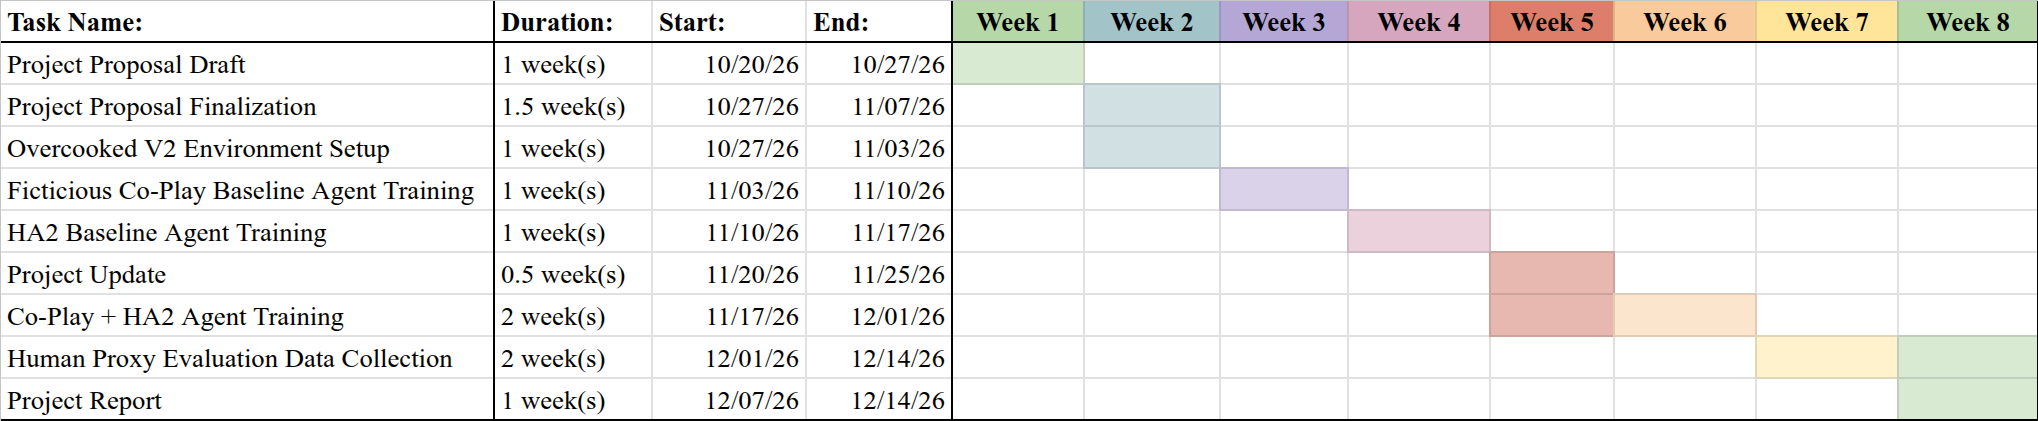
\includegraphics[width=0.9\textwidth]{images/GantChart.png}
    \caption{Gantt chart for the project timeline.}
\end{figure}

\section{What are the mid-term and final ``exams'' to check for success?}

\subsection{Mid-term ``Exam''}

By mid-term, we aim to have a working V2 environment with HA$^2$/FCP baselines for human co-play, an initial teammate intent predictor, and a workflow for reviewing rollouts and collecting sub-task labels or behavioral suggestions.

\subsection{Final ``Exam''}

Our final agent will combine HA$^2$/FCP, human proxies in the partner pool, intent prediction, and human-guided fine-tuning.  We will compare three approaches: the HA$^2$/FCP baseline, an intent-aware variant without direct human feedback, and the full model with feedback.  Evaluation will measure team performance with humans and held-out agent partners, intent prediction accuracy, and human feedback effort, including where the additions help or fail.
Our evaluation will primarily use the environment's cumulative game reward, which rewards correct dish deliveries and penalizes incorrect ones, across multiple trials with human players and held-out agent partners. We will also evaluate intent prediction accuracy using labeled gameplay trajectories. Additionally, to evaluate the collaboration of the agent and human, we will be evaluating the percentages of each recipe that each partner completes in aggregate.  Ideally, a fully cooperative team would have a high percentage of each recipe completed by both partners. Finally, Human participants will complete the NASA Task Load Index (TLX)\cite{hart_development_1988} to evaluate the task load associated with working with the agent as well as the Trust Perception Scale-HRI\cite{schaefer_measuring_2016}.  These results will be compared across the three approaches to determine whether intent prediction and human feedback improve human-agent collaboration.

\newpage
\bibliography{irl_references}

\end{document}
